% options:
% thesis=B bachelor's thesis
% thesis=M master's thesis
% czech thesis in Czech language
% english thesis in English language

\documentclass[thesis=M,czech]{FITthesis}[2012/04/01]

\usepackage[utf8]{inputenc} % LaTeX source encoded as UTF-8

\usepackage{graphicx} %graphics files inclusion
% \usepackage{amsmath} %advanced maths
% \usepackage{amssymb} %additional math symbols

\usepackage{dirtree} %directory tree visualisation

% % list of acronyms
% \usepackage[acronym,nonumberlist,toc,numberedsection=autolabel]{glossaries}
% \iflanguage{czech}{\renewcommand*{\acronymname}{Seznam pou{\v z}it{\' y}ch zkratek}}{}
% \makeglossaries

\newcommand{\tg}{\mathop{\mathrm{tg}}} %cesky tangens
\newcommand{\cotg}{\mathop{\mathrm{cotg}}} %cesky cotangens

% % % % % % % % % % % % % % % % % % % % % % % % % % % % % % 
% ODTUD DAL VSE ZMENTE
% % % % % % % % % % % % % % % % % % % % % % % % % % % % % % 

\department{Katedra softwarového inženýrství}
\title{Webová aplikace pro správu a organizaci nákupního seznamu}
\author{Tomáš Vik} %jméno autora bez akademických titulů
\authorWithDegrees{Bc. Tomáš Vik} %jméno autora včetně akademických titulů
\supervisor{Ing. Jiří Hunka}
\acknowledgements{Sem přijde poděkování.}
\abstractCS{Práce pojednává o problematice nákupních seznamů, dále popisuje návrh a implementaci webové aplikace, která slouží jako pokročilý nákupní seznam.}
\abstractEN{Sem doplňte ekvivalent abstraktu Vaší práce v~angličtině.}
\placeForDeclarationOfAuthenticity{V~Praze}
\keywordsCS{seznam, zboží, prioritizace}
\keywordsEN{list, goods, prioritization}

\begin{document}

% \newacronym{CVUT}{{\v C}VUT}{{\v C}esk{\' e} vysok{\' e} u{\v c}en{\' i} technick{\' e} v Praze}
% \newacronym{FIT}{FIT}{Fakulta informa{\v c}n{\' i}ch technologi{\' i}}

% !TEX root = ../DP_Vik_Tomas_2013.tex
\begin{introduction}
V dnešní době je běžné, že se zákazník před koupí produktu informuje na internetu na cenu v různých obchodech. Dříve musel na internetu použít běžný fulltextový vyhledávač a každý nalezený výsledek produktu musel rozkliknout a nalézt cenu umístěnou na stránce obchodu.

Protože se jedná o relativně složitý proces, vznikly tzv. systémy pro srovnávání cen. Ty odstraňují nutnost hledat cenu výrobku v různých zdrojích. Díky tomu může zákazník přijít na stránku srovnávače cen, nalézt produkt, který chce koupit a poté na jedné přehledné stránce vidí nejen informace o produktu, ale také srovnání cen ve všech srovnávači dostupných obchodech.

Přesto že srovnávání cen je pro zákazníka usnadnění. Cílem této práce je poskytnou další kroky pro zjednodušení nákupu. Práce si klade za cíl navrhnout a vytvořit aplikaci, do které bude zákazníkovi umožněno vložit seznam zboží, které si přeje zakoupit. Takový seznam už některé srovnávače také podporují, ne však s dostatečnou funkcionalitou.

Uživatel bude mít možnost toto zboží (ve zbytku práce nazývané přání) v seznamu kategorizovat, prioritizovat a různými způsoby upravovat. Aplikace dále nejen že bude u těchto přání zobrazovat vývoj ceny, ale navíc dokáže uživatele upozornit na výraznou změnu v tomto vývoji.

V práci budou nejprve detailně zpracovány vlastnosti aplikací s podobnou myšlenkou a dále vlastnosti srovnávačů cen. Na zákaldě této rešerše bude navržena samotná aplikace. Při návrhu bude kladen důraz především na návrh grafického uživatelského rozhranní, které by mělo být intuitivní a usnadňovat uživateli co nejvíce jeho práci.

Dále je krátce popsána zajímavá část implementace a na koneci práce je uživatelské vyhodnocení návrhu grafického rozhraní.
\end{introduction}
% !TEX root = ../viktomas-master.tex
% pokyny
% Z uživatelského hlediska je velmi výhodné před nákupem zboží prozkoumat trh pomocí internetových srovnávačů. Zatím ovšem není snadno dostupná služba, která by uživateli umožnila vytvořit si hypotetický seznam zboží, které zvažuje koupit.

% *Vytvořte rešerši stávajících systémů zabývajících se organizací nákupních seznamů.
% *Zjistěte možnosti a strategii napojení na systémy zabývající se srovnáním a sledováním cen.
% *V souladu s touto rešerší poté analyzujte, navrhněte a implementujte webovou aplikaci, která bude umožňovat přidávat, sledovat, prioritizovat a kategorizovat zboží, zobrazovat jeho cenu a její vývoj.
% *Webovou aplikaci implementujte v jazyce Ruby ve vhodném frameworku.
% *Pro prioritizaci navrhněte a implementujte vhodné algoritmy.
% *API webové aplikace bude navrženo s ohledem na budoucí integraci s dalšími systémy (např. srovnávače cen apod.).
\chapter{Rešerše}
Tato kapitola se zabývá popisem problematiky této práce. V zadání práce je řečeno, že má být vytvořena rešerše stávajících systémů zabývajících se organizací nákupního seznamu. Tato rešerše je rozdělena na 3 kapitoly z nichž každá řeší jeden aspekt těchto seznamů.

\section{Nákupní seznamy}

\subsection{Google ShoppingList}
Webová aplikace založená na službě Google Nákupy. Podporuje jednoduché přidání zboží. U přidaných položek zobrazuje následující informace a umožňuje podle nich i řadit:
\begin{itemize}
\item Datum přidání položky
\item Nejnižší aktuální cena
\item Hodnocení ostatních uživatelů
\end{itemize}
Nákupní seznam je v základním nastavení veřejný a je možné zkopírovat na něj odkaz. Tento odkaz následně uživatel odešle komukoli, s kým chce svůj nákupní seznam sdílet. U každé položky na seznamu je možné vypnout sdílení.

Další funkčnost, kterou nabízí tento seznam je:
\begin{itemize}
\item Přidání poznámky k položce - uživateli je umožněno přidat poznámku k položce na seznamu.  Tato poznámka je následně zobrazena u položky v hlavním přehledu.
\item Odebrání položky ze seznamu
\item Zrušení sdílení - viz. předchozí odstavec
\end{itemize}

\begin{figure}[htb]
\begin{center}
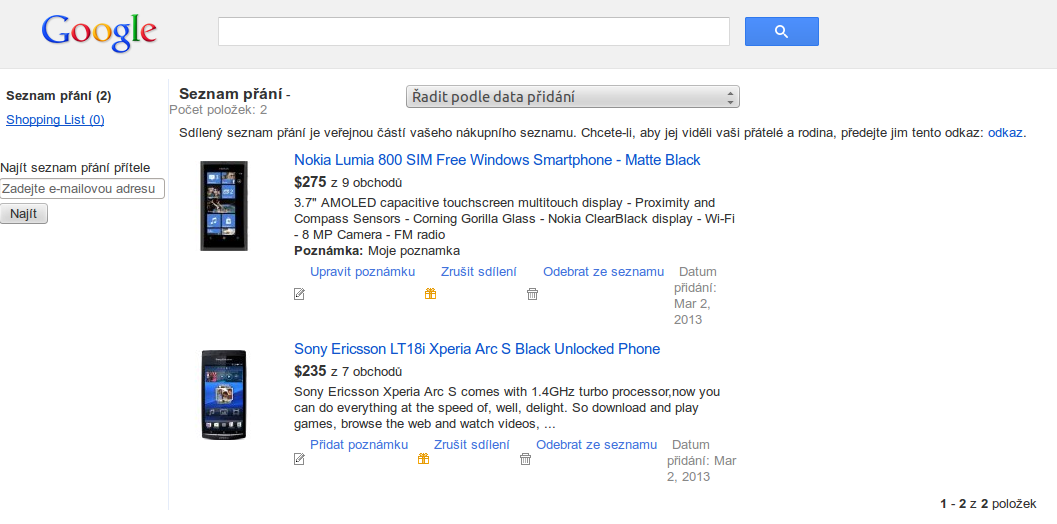
\includegraphics[width=120mm]{./pictures/google-shopping-list.png}
\caption{Google ShoppingList - základní obrazovka}
\label{fig:google-shoppinglist}
\end{center}
\end{figure}

\subsection{Amazon Wish List}
Amazon Wish List je funkcionalita poskytovaná komplementárně k internetovému obchodu Amazon.com. Služba umožňuje vytvářet a sdílet seznamy přání. Pro využívání této služby musí být uživatel přihlášen. Pokud se nepřihlášený uživatel pokusí přidat nějaký předmět do seznamu přání, je přesměrován na stránku přihlášení.

\subsubsection{Druhy přání}
Tato sekce se zabývá druhy přání ve službě Amazon Wish List. Přáním se v této službě rozumí tři věci:
\begin{itemize}
\item Produkt z internetového obchodu Amazon.com
\item Internetová stránka mimo Amazon.com
\item Nápad na přání (tzv. idea)
\end{itemize}

\paragraph{Produkt internetového obchodu Amazon.com}
Toto přání reprezentuje 1:1 produkt v internetovém obchodu Amazon.com. Toto přání vznikne tak, že přihlášený uživatel klikne na stránce produktu na tlačítko "Add To Wish List". U takovéhoto přání se ukazuje minimální možná cena, popis i obrázek.

\paragraph{Internetová stránka mimo Amazon.com}
Toto přání reprezentuje jakoukoli internetovou stránku. Přání vznikne pomocí pluginu Amazon Wish List Button. O této funkcionalitě bude pojednávat samostatná kapitola.

\paragraph{Nápad na přání}
Nápad na přání je funkcionalita, která umožní uživateli zadat nápad na přání pouze jako text (název přání). Tento nápad se uloží mezi ostatní přání. Místo obrázku přání je ovšem zobrazen obrázek nalepovacího štítku a na něm je napsáno "I Want". Nápad na přání je vidět na obrázku \ref{fig:amazon-wishlist-idea}. Každý nápad na přání má u sebe tlačítko "Top search results" které najde pro popis nápadu produkty z obchodu Amazon.com.

\begin{figure}[htb]
\begin{center}
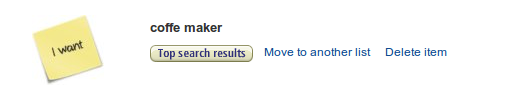
\includegraphics[width=100mm]{./pictures/amazon-wishlist-idea.png}
\caption{Nápad na přání v Amazon Wish List}
\label{fig:amazon-wishlist-idea}
\end{center}
\end{figure}

\subsubsection{Amazon Wish List Button}
Amazon Wish List poskytuje plugin\footnote{Také zásuvný modul - software, který nepracuje samostatně, ale jako doplňkový modul jiné aplikace a rozšiřuje její funkčnost.} do všech majoritních internetových prohlížečů\cite{website:amazon:plugin}. Po nainstalovani pluginu do prohlížeče si může uživatel přidat tlačítko "Amazon Wish List Button". Po stisku tohoto tlačítka se otevře dialog. (Obrázek \ref{fig:amazon-wishlist-plugin})

\begin{figure}[htb]
\begin{center}
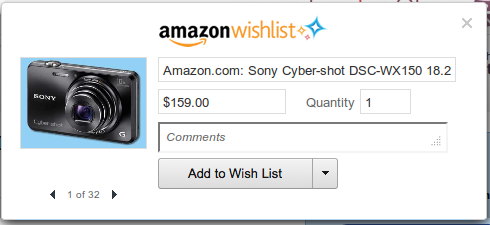
\includegraphics[width=100mm]{./pictures/amazon-wishlist-plugin.png}
\caption{Dialog zobrazeny po stisku Amazon Wish List Button}
\label{fig:amazon-wishlist-plugin}
\end{center}
\end{figure}

Přidat je možné buď produkt z obchodu Amazon. V tomto případě se načtou všechna data, která se u přání ukladájí, a není rozdíl v použití pluginu oproti stisknutí tlačítka "Add to Wish List" na stránce produktu.

Dále plugin podporuje funkci přidání přání v podobě jakékoli stránky. Tedy je možné přidat do Amazon Wish List například zboží z českého internetového obchodu. Jako obrázek k přání si uživatel může zvolit libovolý obrázek ze stránky. Jako název přání se použije titulek stránky\footnote{Obsah HTML tagu <title> ve zdrojovém kódu stránky}, popisek se k přání žádný nepřidává. Uživatel si ještě k přání muže doplnit cenu před tím než ho uloží do seznamu.

\subsection{WishList.com}
WishList.com je webová aplikace zaměřená primárně na vytváření seznamu přání. U každého seznamu podporuje sdílení a také podporuje nastavení události k seznamu a data této události. Většina seznamů má tyto hodnoty vyplněny a jsou to například seznamy přání k narozeninám, vánocům nebo seznam svatebních darů.

WishList.com neumožňuje přihlášení pomocí OpenID. Uživatel se může přihlásit pomocí svého Facebook účtu, nebo zaregistrovat klasickou metodou, kdy zadá svůj email, přihlašovací jméno a heslo.

Uživatel může vytvářet nové seznamy přání a nová přání. Při vytvoření nového seznamu zadává uživatel název seznamu, obrázek seznamu, omezení přístupu (veřejný, pouze přátelé, soukromý), popis seznamu, osobní poznámky, osobu, která si věci přeje, název a datum události. Pouze název seznamu je povinné pole. Seznam je navíc možné zabezpečit heslem.

Při přidávání přání je možné zadat prodejce předmětu, název předmětu, popis předmětu, cenu, množství, prioritu, poznámky k přání, seznam přání do kterého bude přání přidáno, příjemce přání a poté URL produktu a URL obrázku produktu. Povinným polem je pouze název předmětu.

Vytvořený seznam je možné sdílet pomocí URL. Pokud si seznam prohlíží jiný uživatel než ten, který jej vytvořil, může si tento uživatel zarezervovat přání, což znamená že koupí předmět a dá jej uživateli, který si jej přál.

Seznam přání i jednotlivá přání je možné sdílet s ostatními uživateli pomocí tlačitka "Share this WishList" resp "Share this Wish". Sdílení j e možné pomocí služeb Facebook, Myspace, Google, Twitter, Email a dalších 300+. Na sdílení je pravděpodobně použit nějaký plugin.

Přehled přání je vidět na obrázku \ref{fig:wishlist-wishlist}

\begin{figure}[htb]
\begin{center}
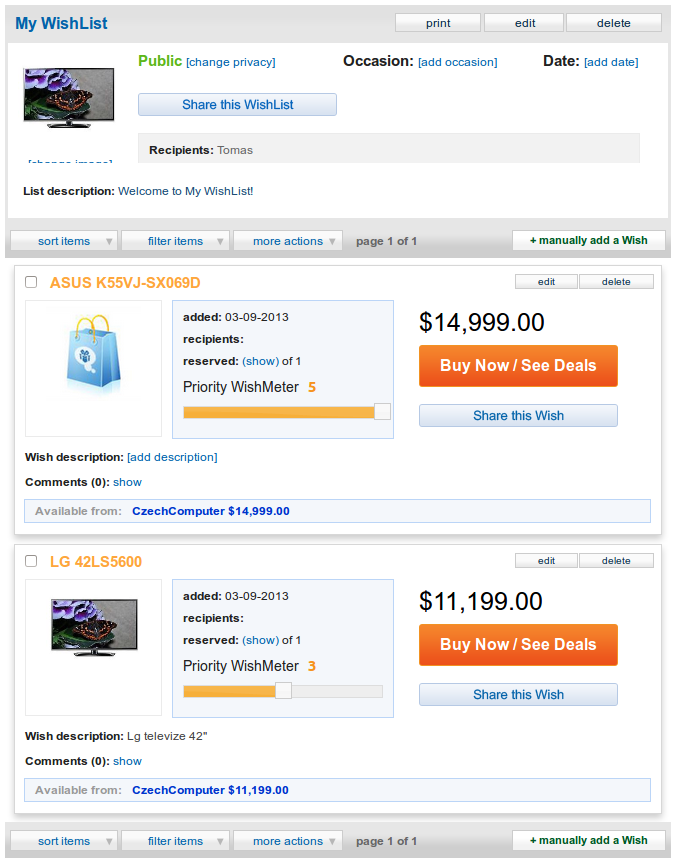
\includegraphics[width=100mm]{./pictures/wishlist-wishlist.png}
\caption{Hlavní přehled přání na stránce WishList.com}
\label{fig:wishlist-wishlist}
\end{center}
\end{figure}

\section{Srovnávače cen}
Tato kapitola poskytuje rešerši produktů známých jako srovnávače cen. Cílem těchto produktů je poskytnout uživateli širší rozhled na trh. Tyto produkty umožňují u jednoho druhu zboží (např. Televizor) srovnat jeho cenu v několika obchodech. V rešerši jsou zpracovány jako potencionální zdroje dat pro nákupní seznam.

\subsection{Standartní funkce všech srovnávačů}
V této sekci jsou popsány 3 základní funkce, které podporují všechny srovnávače cen.

\subsubsection{Vyhledávání}
Každý ze zmíňených vyhledávačů podporuje fultextové vyhledávání zboží. Dále umožňují srovnávače vyhledávání po kategoriích a/nebo filtrování parametrů zboží.

\subsubsection{Srovnávání cen}
Každý z vyhledávačů podporuje srovnání cen u zobží. U každého zboží je schopný zobrazit minimální cenu a také seznam všech obchodů s tímto zbožím a k nim přiřazenou částku, za jakou daný obchod zboží nabízí.

K této funkcionalitě zároveň patří graf historie cen. V grafu historie cen uživatel může sledovat vývoj ceny zboží a třeba odhadnout, jak se bude vyvíjet dál.

\subsubsection{Uživatelská zpětná vazba}
Touto funkčností se rozumí uživatelské hodnocení produktů a obchodů. Hodnocení většinou probíhá na principu jedné až pěti hvězdiček, případně shrnutí kladů a záporů.

\subsection{Heureka}
Interaktivní nákupní rádce Heureka.cz byl založen společností Miton v roce 2007, kdy ihned zaujmul zajímavým nápadem zkombinování mnoha užitečných možností do jednoho celku. Následně rozšiřuje svou působnost i na Slovensko a zakládá slovenskou verzi Heureka.sk (založena v r. 2008). \cite{website:wiki:heureka}

\subsubsection{Funkčnost nad rámec základní funkčnosti}
Další důležitou fukčností je hlídač ceny. Přihlášenému uživateli je umožněno na zboží nastavit hlídače ceny a poté co cena v nejlevnějším obchodě klesne pod zadanou částku, uživatel dostane email s upozorněním.

\begin{itemize}
\item Záruka vrácení peněz u některých obchodů
\item Varování před obhody, které nedodržují své obchodní podmínky
\item Sledovaní slev a novinek na trhu
\end{itemize}
\subsection{Zboží.cz}
Zboží.cz je satelitní web společnosti Seznam.cz
\footnote{Satelitní web je rozšířená a propracovanější forma tzv. microsite (jinak také minisite či weblet), jde o speciální samostatný web plnící funkce, které se na hlavní webovou prezentaci nehodí, nebo s ní dokonce nesouvisejí.}
. 

%\section{NextTag}
% \section{WunderList}

\subsection{PriceGrabber}
PriceGrabber je služba pro srovnávání cen. Jejími partnery je více než 13000 prodejců. Poskytuje volně informace o milionech produktů ve více než 25 kategoriích. Společnost také slouží jako datový zdroj pro další prodejní služby jako AOL Shopping, Bing Shopping aj. \cite{website:wiki:pricegrabber}

Price grabber byl první srovnávač, který zahrnul informace o daních a poplatcích za přepravu do srovnávání. \cite{website:wiki:pricegrabber}
% !TEX root = ../DP_Vik_Tomas_2013.tex
\begin{conclusion}

Moderní webové aplikace na srovnávání a nakupování popsané v rešerši jsou pro zákazníka ohromnou úsporou času a peněz při nakupování. Výsledná aplikace se snažila stavět na přidané hodnotě těchto webových aplikací a jít ještě dále v usnadnění uživatelovi činnosti.

V práci byla nalezena funkcionalita, která je běžně poskytována současnými aplikacemi a dále bylo navrženo několik funkcí, díky kterým bude výsledný seznam přání pro uživatele užitečný.

Při návrhu uživatelského rozhranní bylo postupováno v souladu s Nielsenovou heuristikou\cite{molich1990improving}. A všeobecně byl kladen velký důraz na jednoduchost UI.

Implementace proběhla v nejmodernějších technologiích, což se příznivě podepsalo na vzhledu uživatelského rozhraní, jako například dynamické donačítání dat do stránek, mnoho javascriptových modálních oken atp. Vybraná metoda získávání dat (Web Scraping) sebou přinesla jak výhody, tak několik nevýhod a to především menší interaktivitu se zdrojem dat, kvůli snaze o malé zatěžování serveru aplikace pro srovnávání cen.

Závěrečnou zkouškou aplikace bylo uživatelské testování provedené formou dotazníku pro snadnou kvantifikaci výsledků. Z tohoto testování vyplynuly následující závěry. Aplikace má dobré až výborné uživatelské rozhranní, což bylo ověřeno pomocí SUS dotazníku. Návrh UI přesto nebyl zdaleka bezchybný, což se ukázalo v části dotazníku zaměřeném na konkrétní funkce aplikace. Pro několik funkcí bylo uživatelské rozhranní navržené nedostatečně výrazně a uživatelé tyto funkce přehlédli. Dokonce ani navržení dotazníku se neobešlo bez chyby a dvě otázky se ukázaly nešťastně zforulované.

Celkově práce splnila své zadání a poskytla jedinečný pohled na systémy srovnávání cen a funkcionalitu, kterou je možné tyto velké databáze rozšířit a obohatit tak uživatelovu zkušenost.


\end{conclusion}

\bibliographystyle{csn690}
\bibliography{viktomas_master}

\appendix

\chapter{Seznam použitých zkratek}
% \printglossaries
\begin{description}
	\item[GUI] Graphical user interface
	\item[XML] Extensible markup language
	\item[URL] Unified Resource Locator
\end{description}


% % % % % % % % % % % % % % % % % % % % % % % % % % % % 
% % Tuto kapitolu z výsledné práce ODSTRAŇTE.
% % % % % % % % % % % % % % % % % % % % % % % % % % % % 
% 
% \chapter{Návod k~použití této šablony}
% 
% Tento dokument slouží jako základ pro napsání závěrečné práce na Fakultě informačních technologií ČVUT v~Praze.
% 
% \section{Výběr základu}
% 
% Vyberte si šablonu podle druhu práce (bakalářská, diplomová), jazyka (čeština, angličtina) a kódování (ASCII, \mbox{UTF-8}, \mbox{ISO-8859-2} neboli latin2 a nebo \mbox{Windows-1250}). 
% 
% V~české variantě naleznete šablony v~souborech pojmenovaných ve formátu práce\_kódování.tex. Typ může být:
% \begin{description}
% 	\item[BP] bakalářská práce,
% 	\item[DP] diplomová (magisterská) práce.
% \end{description}
% Kódování, ve kterém chcete psát, může být:
% \begin{description}
% 	\item[UTF-8] kódování Unicode,
% 	\item[ISO-8859-2] latin2,
% 	\item[Windows-1250] znaková sada 1250 Windows.
% \end{description}
% V~případě nejistoty ohledně kódování doporučujeme následující postup:
% \begin{enumerate}
% 	\item Otevřete šablony pro kódování UTF-8 v~editoru prostého textu, který chcete pro psaní práce použít -- pokud můžete texty s~diakritikou normálně přečíst, použijte tuto šablonu.
% 	\item V~opačném případě postupujte dále podle toho, jaký operační systém používáte:
% 	\begin{itemize}
% 		\item v~případě Windows použijte šablonu pro kódování \mbox{Windows-1250},
% 		\item jinak zkuste použít šablonu pro kódování \mbox{ISO-8859-2}.
% 	\end{itemize}
% \end{enumerate}
% 
% 
% V~anglické variantě jsou šablony pojmenované podle typu práce, možnosti jsou:
% \begin{description}
% 	\item[bachelors] bakalářská práce,
% 	\item[masters] diplomová (magisterská) práce.
% \end{description}
% 
% \section{Použití šablony}
% 
% Šablona je určena pro zpracování systémem \LaTeXe{}. Text je možné psát v~textovém editoru jako prostý text, lze však také využít specializovaný editor pro \LaTeX{}, např. Kile.
% 
% Pro získání tisknutelného výstupu z~takto vytvořeného souboru použijte příkaz \verb|pdflatex|, kterému předáte cestu k~souboru jako parametr. Vhodný editor pro \LaTeX{} toto udělá za Vás. \verb|pdfcslatex| ani \verb|cslatex| \emph{nebudou} s~těmito šablonami fungovat.
% 
% Více informací o~použití systému \LaTeX{} najdete např. v~\cite{wikilatex}.
% 
% \subsection{Typografie}
% 
% Při psaní dodržujte typografické konvence zvoleného jazyka. České \uv{uvozovky} zapisujte použitím příkazu \verb|\uv|, kterému v~parametru předáte text, jenž má být v~uvozovkách. Anglické otevírací uvozovky se v~\LaTeX{}u zadávají jako dva zpětné apostrofy, uzavírací uvozovky jako dva apostrofy. Často chybně uváděný symbol "{} (palce) nemá s~uvozovkami nic společného.
% 
% Dále je třeba zabránit zalomení řádky mezi některými slovy, v~češtině např. za jednopísmennými předložkami a spojkami (vyjma \uv{a}). To docílíte vložením pružné nezalomitelné mezery -- znakem \texttt{\textasciitilde}. V~tomto případě to není třeba dělat ručně, lze použít program \verb|vlna|.
% 
% Více o~typografii viz \cite{kobltypo}.
% 
% \subsection{Obrázky}
% 
% Pro umožnění vkládání obrázků je vhodné použít balíček \verb|graphicx|, samotné vložení se provede příkazem \verb|\includegraphics|. Takto je možné vkládat obrázky ve formátu PDF, PNG a JPEG jestliže používáte pdf\LaTeX{} nebo ve formátu EPS jestliže používáte \LaTeX{}. Doporučujeme preferovat vektorové obrázky před rastrovými (vyjma fotografií).
% 
% \subsubsection{Získání vhodného formátu}
% 
% Pro získání vektorových formátů PDF nebo EPS z~jiných lze použít některý z~vektorových grafických editorů. Pro převod rastrového obrázku na vektorový lze použít rasterizaci, kterou mnohé editory zvládají (např. Inkscape). Pro konverze lze použít též nástroje pro dávkové zpracování běžně dodávané s~\LaTeX{}em, např. \verb|epstopdf|.
% 
% \subsubsection{Plovoucí prostředí}
% 
% Příkazem \verb|\includegraphics| lze obrázky vkládat přímo, doporučujeme však použít plovoucí prostředí, konkrétně \verb|figure|. Například obrázek \ref{fig:float} byl vložen tímto způsobem. Vůbec přitom nevadí, když je obrázek umístěn jinde, než bylo původně zamýšleno -- je tomu tak hlavně kvůli dodržení typografických konvencí. Namísto vynucování konkrétní pozice obrázku doporučujeme používat odkazování z~textu (dvojice příkazů \verb|\label| a \verb|\ref|).
% 
% \begin{figure}\centering
% 	
\includegraphics[width=0.5\textwidth, angle=30]{cvut-logo-bw}
% 	\caption[Příklad obrázku]{Ukázkový obrázek v~plovoucím prostředí}\label{fig:float}
% \end{figure}
% 
% \subsubsection{Verze obrázků}
% 
% % Gnuplot BW i barevně
% Může se hodit mít více verzí stejného obrázku, např. pro barevný či černobílý tisk a nebo pro prezentaci. S~pomocí některých nástrojů na generování grafiky je to snadné.
% 
% Máte-li například graf vytvořený v programu Gnuplot, můžete jeho černobílou variantu (viz obr. \ref{fig:gnuplot-bw}) vytvořit parametrem \verb|monochrome dashed| příkazu \verb|set term|. Barevnou variantu (viz obr. \ref{fig:gnuplot-col}) vhodnou na prezentace lze vytvořit parametrem \verb|colour solid|.
% 
% \begin{figure}\centering
% 	\includegraphics{gnuplot-bw}
% 	\caption{Černobílá varianta obrázku generovaného programem Gnuplot}\label{fig:gnuplot-bw}
% \end{figure}
% 
% \begin{figure}\centering
% 	\includegraphics{gnuplot-col}
% 	\caption{Barevná varianta obrázku generovaného programem Gnuplot}\label{fig:gnuplot-col}
% \end{figure}
% 
% 
% \subsection{Tabulky}
% 
% Tabulky lze zadávat různě, např. v~prostředí \verb|tabular|, avšak pro jejich vkládání platí to samé, co pro obrázky -- použijte plovoucí prostředí, v~tomto případě \verb|table|. Například tabulka \ref{tab:matematika} byla vložena tímto způsobem.
% 
% \begin{table}\centering
% 	\caption[Příklad tabulky]{Zadávání matematiky}\label{tab:matematika}
% 	\begin{tabular}{|l|l|c|c|}\hline
% 		Typ		& Prostředí		& \LaTeX{}ovská zkratka	& \TeX{}ovská zkratka	\tabularnewline \hline \hline
% 		Text		& \verb|math|		& \verb|\(...\)|	& \verb|$...$|		\tabularnewline \hline
% 		Displayed	& \verb|displaymath|	& \verb|\[...\]|	& \verb|$$...$$|	\tabularnewline \hline
% 	\end{tabular}
% \end{table}
% 
% % % % % % % % % % % % % % % % % % % % % % % % % % % % 

\chapter{Obsah přiloženého CD}

%upravte podle skutecnosti

\begin{figure}
	\dirtree{%
		.1 readme.txt\DTcomment{stručný popis obsahu CD}.
		.1 exe\DTcomment{adresář se spustitelnou formou implementace}.
		.1 src.
		.2 impl\DTcomment{zdrojové kódy implementace}.
		.2 thesis\DTcomment{zdrojová forma práce ve formátu \LaTeX{}}.
		.1 text\DTcomment{text práce}.
		.2 thesis.pdf\DTcomment{text práce ve formátu PDF}.
		.2 thesis.ps\DTcomment{text práce ve formátu PS}.
	}
\end{figure}

\end{document}
